%%%%%%%%%%%%%%%%%%%%%%%%%%%%%%%%%%%%%%%%%%%%%%%%%%%%%%%%%%%%%%%%%%%%%%
% This layout was adapted from one found at latextemplates.com which
% was adapted from another.
%
% License: CC BY-NC-SA 3.0
% (http://creativecommons.org/licenses/by-nc-sa/3.0/)
%
% Original header:
%
% This is a LaTeX version of the sample laboratory report from
% Virginia Tech's copyrighted 08-09 CHEM 1045/1046 lab manual.
% Reproduction of this one appendix section for academic purposes
% should fall under fair use.
%
%%%%%%%%%%%%%%%%%%%%%%%%%%%%%%%%%%%%%%%%%%%%%%%%%%%%%%%%%%%%%%%%%%%%%%

\documentclass{article}

\usepackage{graphicx}
%\usepackage[acronym]{glossaries} % Lets us use acronyms
\usepackage{multicol}
\usepackage{siunitx} % SI units in math mode

\author{}
\title{ELEC-313 \\ Lab 2: Diode Characterization \\ }
\date{\today}

%\loadglsentries{acronyms} % Actually loads 'acronyms.tex'
%\makeglossaries

\begin{document}

\maketitle

\begin{center}
  \begin{tabular}{lr}
    Date Performed: & September 18, 2013 \\
    Partners: & Charles Pittman \\
    & Stephen Wilson \\
  \end{tabular}
\end{center}

\pagebreak

% Removes indentation from paragraphs: \setlength\parindent{0pt}

% Number the enumerate environment (unordered lists) by letter:
\renewcommand{\labelenumi}{\alph{enumi}.}

\section{Objective}
\label{sec:objective}

The objective is to observe the basic operation of a diode.  In
addition, the Schlockley equation (Eq~\ref{eqn:schlockley}) is used to
find the diode's reverse saturation current ($I_S$) and thermal
voltage ($V_T$) using values measured in the lab.

\section{Equipment}
\label{sec:equipment}

%\begin{multicols}{2}
%  \begin{description}
%  \item[Diode] \hfill \\ 1N4002
%  \item[Resistors] \hfill \\ \SI{330}{\ohm}, \SI{470}{\ohm}, \SI{680}{\ohm}
%  \item[Resistive Decade box] \hfill \\ Heathkit IN--3117
%  \item[Power supply] \hfill \\ HP E3631A
%  \item[Multimeter] \hfill \\ Fluke 8010A
%  \end{description}
%\end{multicols}

\begin{tabular}{ll}
  \centering
  Diode: 1N4002 & Power supply: HP E3631A \\
  Resistors: \SI{330}{\ohm}, \SI{470}{\ohm}, \SI{680}{\ohm} & Multimeter: Fluke 8010A (x2)\\
  Resistive decade box: HeathKit IN-3117 & \\
\end{tabular}

\section{Schematics}
\label{sec:schematics}

\subsection{Circuits Tested}
\label{sec:ckt_tested}

\begin{figure}[hbtp]
  \centering
  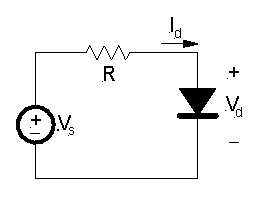
\includegraphics[]{img/circuit1}
  \caption{\label{fig:circuit1} Circuit used for Part A and Part B.}
\end{figure}

\begin{figure}[hbtp]
  \centering
  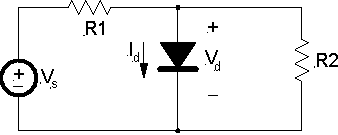
\includegraphics[]{img/circuit2}
  \caption{\label{fig:circuit2} Circuit used for Part C.}
\end{figure}

\section{Procedure}
\label{sec:procedure}

\subsection{Part A}
\label{sec:proc_a}

The circuit in Figure~\ref{fig:circuit1} was constructed, with $R =
\SI{470}{\ohm}$ and the power supply as $V_s$.  The actual resistance
was measured with one a multimeter and recorded in
Table~\ref{tab:percent_err} along with the percent error calculated
(Eq~\ref{eqn:percent_err}).  Next, the multimeters were used to
measure voltage across and current through the diode ($V_d$ and $I_d$,
respectively) while $V_s$ was swept from \SI{-5}{V} to \SI{+10}{V}.
The step size from \SI{-5}{V} to \SI{0}{V} and from \SI{5}{V} to
\SI{10}{V} was \SI{0.5}{V}, and \SI{0.25}{V} from \SI{0}{V} to
\SI{5}{V}.  These values were recorded in Table~\ref{tab:part_a} and
used to generate the graph in Figure~\ref{fig:part_a_graph}.

\subsection{Part B}
\label{sec:proc_b}

Lorem ipsum dolor sit amet, consectetuer adipiscing elit. Donec
hendrerit tempor tellus. Donec pretium posuere tellus. Proin quam
nisl, tincidunt et, mattis eget, convallis nec, purus. Cum sociis
natoque penatibus et magnis dis parturient montes, nascetur ridiculus
mus. Nulla posuere. Donec vitae dolor. Nullam tristique diam non
turpis. Cras placerat accumsan nulla. Nullam rutrum. Nam vestibulum
accumsan nisl.

\subsection{Part C}
\label{sec:proc_c}

Lorem ipsum dolor sit amet, consectetuer adipiscing elit. Donec
hendrerit tempor tellus. Donec pretium posuere tellus. Proin quam
nisl, tincidunt et, mattis eget, convallis nec, purus. Cum sociis
natoque penatibus et magnis dis parturient montes, nascetur ridiculus
mus. Nulla posuere. Donec vitae dolor. Nullam tristique diam non
turpis. Cras placerat accumsan nulla. Nullam rutrum. Nam vestibulum
accumsan nisl.

In part B, the 470 ohm resistor (Figure 1) was replaced with
a 200 resistor using a decade box and Vs (Figure 1) was set to 10V and
Vd and the Id were measured and recorded in Table 1. The decade box
was adjust with the voltages listed in Table 1 by adjusting the decade
box , and the Vd and the Id were measured and recorded for each
setting of resistance.  In part C of the experiment, the circuit in
Figure 2 was built on a breadboard using the HP power supply as the
Vs. Vd and the Id were measured and recorded in Table 2. The diode was
then removed and the open circuit voltage (VOC) was recorded (Table
2).

\section{Results}
\label{sec:results}

\subsection{Part A}
\label{sec:result_a}

\begin{table}[hbtp]
  \centering
  \begin{tabular}{*{4}{c}}
    \textbf{Name} & \textbf{Nominal} & \textbf{Measured} & \textbf{\% Error} \\
    & (\si{\ohm}) & (\si{\ohm}) & \\
    \hline
    $R_1$ & 470 & 465.3 & 1.00 \\
  \end{tabular}
  \caption{\label{tab:percent_err} Comparison of nominal and measured resistance in Part A.}
\end{table}

\begin{figure}[hbtp]
  \centering
  % GNUPLOT: LaTeX picture
\setlength{\unitlength}{0.240900pt}
\ifx\plotpoint\undefined\newsavebox{\plotpoint}\fi
\begin{picture}(1500,900)(0,0)
\sbox{\plotpoint}{\rule[-0.200pt]{0.400pt}{0.400pt}}%
\put(151.0,131.0){\rule[-0.200pt]{4.818pt}{0.400pt}}
\put(131,131){\makebox(0,0)[r]{ 0}}
\put(1419.0,131.0){\rule[-0.200pt]{4.818pt}{0.400pt}}
\put(151.0,196.0){\rule[-0.200pt]{4.818pt}{0.400pt}}
\put(131,196){\makebox(0,0)[r]{ 2}}
\put(1419.0,196.0){\rule[-0.200pt]{4.818pt}{0.400pt}}
\put(151.0,260.0){\rule[-0.200pt]{4.818pt}{0.400pt}}
\put(131,260){\makebox(0,0)[r]{ 4}}
\put(1419.0,260.0){\rule[-0.200pt]{4.818pt}{0.400pt}}
\put(151.0,325.0){\rule[-0.200pt]{4.818pt}{0.400pt}}
\put(131,325){\makebox(0,0)[r]{ 6}}
\put(1419.0,325.0){\rule[-0.200pt]{4.818pt}{0.400pt}}
\put(151.0,389.0){\rule[-0.200pt]{4.818pt}{0.400pt}}
\put(131,389){\makebox(0,0)[r]{ 8}}
\put(1419.0,389.0){\rule[-0.200pt]{4.818pt}{0.400pt}}
\put(151.0,454.0){\rule[-0.200pt]{4.818pt}{0.400pt}}
\put(131,454){\makebox(0,0)[r]{ 10}}
\put(1419.0,454.0){\rule[-0.200pt]{4.818pt}{0.400pt}}
\put(151.0,518.0){\rule[-0.200pt]{4.818pt}{0.400pt}}
\put(131,518){\makebox(0,0)[r]{ 12}}
\put(1419.0,518.0){\rule[-0.200pt]{4.818pt}{0.400pt}}
\put(151.0,583.0){\rule[-0.200pt]{4.818pt}{0.400pt}}
\put(131,583){\makebox(0,0)[r]{ 14}}
\put(1419.0,583.0){\rule[-0.200pt]{4.818pt}{0.400pt}}
\put(151.0,647.0){\rule[-0.200pt]{4.818pt}{0.400pt}}
\put(131,647){\makebox(0,0)[r]{ 16}}
\put(1419.0,647.0){\rule[-0.200pt]{4.818pt}{0.400pt}}
\put(151.0,712.0){\rule[-0.200pt]{4.818pt}{0.400pt}}
\put(131,712){\makebox(0,0)[r]{ 18}}
\put(1419.0,712.0){\rule[-0.200pt]{4.818pt}{0.400pt}}
\put(151.0,776.0){\rule[-0.200pt]{4.818pt}{0.400pt}}
\put(131,776){\makebox(0,0)[r]{ 20}}
\put(1419.0,776.0){\rule[-0.200pt]{4.818pt}{0.400pt}}
\put(151.0,131.0){\rule[-0.200pt]{0.400pt}{4.818pt}}
\put(151,90){\makebox(0,0){ 0}}
\put(151.0,756.0){\rule[-0.200pt]{0.400pt}{4.818pt}}
\put(323.0,131.0){\rule[-0.200pt]{0.400pt}{4.818pt}}
\put(323,90){\makebox(0,0){ 0.1}}
\put(323.0,756.0){\rule[-0.200pt]{0.400pt}{4.818pt}}
\put(494.0,131.0){\rule[-0.200pt]{0.400pt}{4.818pt}}
\put(494,90){\makebox(0,0){ 0.2}}
\put(494.0,756.0){\rule[-0.200pt]{0.400pt}{4.818pt}}
\put(666.0,131.0){\rule[-0.200pt]{0.400pt}{4.818pt}}
\put(666,90){\makebox(0,0){ 0.3}}
\put(666.0,756.0){\rule[-0.200pt]{0.400pt}{4.818pt}}
\put(838.0,131.0){\rule[-0.200pt]{0.400pt}{4.818pt}}
\put(838,90){\makebox(0,0){ 0.4}}
\put(838.0,756.0){\rule[-0.200pt]{0.400pt}{4.818pt}}
\put(1010.0,131.0){\rule[-0.200pt]{0.400pt}{4.818pt}}
\put(1010,90){\makebox(0,0){ 0.5}}
\put(1010.0,756.0){\rule[-0.200pt]{0.400pt}{4.818pt}}
\put(1181.0,131.0){\rule[-0.200pt]{0.400pt}{4.818pt}}
\put(1181,90){\makebox(0,0){ 0.6}}
\put(1181.0,756.0){\rule[-0.200pt]{0.400pt}{4.818pt}}
\put(1353.0,131.0){\rule[-0.200pt]{0.400pt}{4.818pt}}
\put(1353,90){\makebox(0,0){ 0.7}}
\put(1353.0,756.0){\rule[-0.200pt]{0.400pt}{4.818pt}}
\put(151.0,131.0){\rule[-0.200pt]{0.400pt}{155.380pt}}
\put(151.0,131.0){\rule[-0.200pt]{310.279pt}{0.400pt}}
\put(1439.0,131.0){\rule[-0.200pt]{0.400pt}{155.380pt}}
\put(151.0,776.0){\rule[-0.200pt]{310.279pt}{0.400pt}}
\put(30,453){\makebox(0,0){\shortstack{$I_d$\\(mA)}}}
\put(795,29){\makebox(0,0){$V_d$ (V)}}
\put(795,838){\makebox(0,0){Diode Current vs. Voltage}}
\put(627,131){\makebox(0,0){$+$}}
\put(587,131){\makebox(0,0){$+$}}
\put(943,134){\makebox(0,0){$+$}}
\put(1071,146){\makebox(0,0){$+$}}
\put(1130,161){\makebox(0,0){$+$}}
\put(1166,176){\makebox(0,0){$+$}}
\put(1192,192){\makebox(0,0){$+$}}
\put(1212,208){\makebox(0,0){$+$}}
\put(1228,225){\makebox(0,0){$+$}}
\put(1242,241){\makebox(0,0){$+$}}
\put(1254,257){\makebox(0,0){$+$}}
\put(1264,274){\makebox(0,0){$+$}}
\put(1272,291){\makebox(0,0){$+$}}
\put(1281,307){\makebox(0,0){$+$}}
\put(1288,324){\makebox(0,0){$+$}}
\put(1295,341){\makebox(0,0){$+$}}
\put(1302,358){\makebox(0,0){$+$}}
\put(1307,374){\makebox(0,0){$+$}}
\put(1312,392){\makebox(0,0){$+$}}
\put(1317,408){\makebox(0,0){$+$}}
\put(1322,425){\makebox(0,0){$+$}}
\put(1331,459){\makebox(0,0){$+$}}
\put(1339,493){\makebox(0,0){$+$}}
\put(1346,528){\makebox(0,0){$+$}}
\put(1351,562){\makebox(0,0){$+$}}
\put(1358,596){\makebox(0,0){$+$}}
\put(1363,631){\makebox(0,0){$+$}}
\put(1369,665){\makebox(0,0){$+$}}
\put(1374,701){\makebox(0,0){$+$}}
\put(1377,736){\makebox(0,0){$+$}}
\put(1382,771){\makebox(0,0){$+$}}
\put(151.0,131.0){\rule[-0.200pt]{0.400pt}{155.380pt}}
\put(151.0,131.0){\rule[-0.200pt]{310.279pt}{0.400pt}}
\put(1439.0,131.0){\rule[-0.200pt]{0.400pt}{155.380pt}}
\put(151.0,776.0){\rule[-0.200pt]{310.279pt}{0.400pt}}
\end{picture}

  \caption{\label{fig:part_a_graph} Diode characteristics measured in Part A.}
\end{figure}

\begin{figure}[hbtp]
  \centering
  % GNUPLOT: LaTeX picture
\setlength{\unitlength}{0.240900pt}
\ifx\plotpoint\undefined\newsavebox{\plotpoint}\fi
\sbox{\plotpoint}{\rule[-0.200pt]{0.400pt}{0.400pt}}%
\begin{picture}(1500,900)(0,0)
\sbox{\plotpoint}{\rule[-0.200pt]{0.400pt}{0.400pt}}%
\put(171.0,131.0){\rule[-0.200pt]{4.818pt}{0.400pt}}
\put(151,131){\makebox(0,0)[r]{ 0}}
\put(1419.0,131.0){\rule[-0.200pt]{4.818pt}{0.400pt}}
\put(171.0,239.0){\rule[-0.200pt]{4.818pt}{0.400pt}}
\put(151,239){\makebox(0,0)[r]{ 0.5}}
\put(1419.0,239.0){\rule[-0.200pt]{4.818pt}{0.400pt}}
\put(171.0,346.0){\rule[-0.200pt]{4.818pt}{0.400pt}}
\put(151,346){\makebox(0,0)[r]{ 1}}
\put(1419.0,346.0){\rule[-0.200pt]{4.818pt}{0.400pt}}
\put(171.0,454.0){\rule[-0.200pt]{4.818pt}{0.400pt}}
\put(151,454){\makebox(0,0)[r]{ 1.5}}
\put(1419.0,454.0){\rule[-0.200pt]{4.818pt}{0.400pt}}
\put(171.0,561.0){\rule[-0.200pt]{4.818pt}{0.400pt}}
\put(151,561){\makebox(0,0)[r]{ 2}}
\put(1419.0,561.0){\rule[-0.200pt]{4.818pt}{0.400pt}}
\put(171.0,669.0){\rule[-0.200pt]{4.818pt}{0.400pt}}
\put(151,669){\makebox(0,0)[r]{ 2.5}}
\put(1419.0,669.0){\rule[-0.200pt]{4.818pt}{0.400pt}}
\put(171.0,776.0){\rule[-0.200pt]{4.818pt}{0.400pt}}
\put(151,776){\makebox(0,0)[r]{ 3}}
\put(1419.0,776.0){\rule[-0.200pt]{4.818pt}{0.400pt}}
\put(171.0,131.0){\rule[-0.200pt]{0.400pt}{4.818pt}}
\put(171,90){\makebox(0,0){ 0}}
\put(171.0,756.0){\rule[-0.200pt]{0.400pt}{4.818pt}}
\put(330.0,131.0){\rule[-0.200pt]{0.400pt}{4.818pt}}
\put(330,90){\makebox(0,0){ 0.1}}
\put(330.0,756.0){\rule[-0.200pt]{0.400pt}{4.818pt}}
\put(488.0,131.0){\rule[-0.200pt]{0.400pt}{4.818pt}}
\put(488,90){\makebox(0,0){ 0.2}}
\put(488.0,756.0){\rule[-0.200pt]{0.400pt}{4.818pt}}
\put(647.0,131.0){\rule[-0.200pt]{0.400pt}{4.818pt}}
\put(647,90){\makebox(0,0){ 0.3}}
\put(647.0,756.0){\rule[-0.200pt]{0.400pt}{4.818pt}}
\put(805.0,131.0){\rule[-0.200pt]{0.400pt}{4.818pt}}
\put(805,90){\makebox(0,0){ 0.4}}
\put(805.0,756.0){\rule[-0.200pt]{0.400pt}{4.818pt}}
\put(964.0,131.0){\rule[-0.200pt]{0.400pt}{4.818pt}}
\put(964,90){\makebox(0,0){ 0.5}}
\put(964.0,756.0){\rule[-0.200pt]{0.400pt}{4.818pt}}
\put(1122.0,131.0){\rule[-0.200pt]{0.400pt}{4.818pt}}
\put(1122,90){\makebox(0,0){ 0.6}}
\put(1122.0,756.0){\rule[-0.200pt]{0.400pt}{4.818pt}}
\put(1281.0,131.0){\rule[-0.200pt]{0.400pt}{4.818pt}}
\put(1281,90){\makebox(0,0){ 0.7}}
\put(1281.0,756.0){\rule[-0.200pt]{0.400pt}{4.818pt}}
\put(1439.0,131.0){\rule[-0.200pt]{0.400pt}{4.818pt}}
\put(1439,90){\makebox(0,0){ 0.8}}
\put(1439.0,756.0){\rule[-0.200pt]{0.400pt}{4.818pt}}
\put(171.0,131.0){\rule[-0.200pt]{0.400pt}{155.380pt}}
\put(171.0,131.0){\rule[-0.200pt]{305.461pt}{0.400pt}}
\put(1439.0,131.0){\rule[-0.200pt]{0.400pt}{155.380pt}}
\put(171.0,776.0){\rule[-0.200pt]{305.461pt}{0.400pt}}
\put(30,453){\makebox(0,0){\shortstack{ln($I_d$)\\(mA)}}}
\put(805,29){\makebox(0,0){$V_d$ (V)}}
\put(805,838){\makebox(0,0){Diode Natural Logarithm of Current vs. Voltage}}
\put(1108,203){\makebox(0,0){$+$}}
\put(1132,268){\makebox(0,0){$+$}}
\put(1151,318){\makebox(0,0){$+$}}
\put(1165,360){\makebox(0,0){$+$}}
\put(1177,395){\makebox(0,0){$+$}}
\put(1189,425){\makebox(0,0){$+$}}
\put(1198,451){\makebox(0,0){$+$}}
\put(1206,475){\makebox(0,0){$+$}}
\put(1214,496){\makebox(0,0){$+$}}
\put(1220,516){\makebox(0,0){$+$}}
\put(1227,534){\makebox(0,0){$+$}}
\put(1233,550){\makebox(0,0){$+$}}
\put(1238,566){\makebox(0,0){$+$}}
\put(1242,580){\makebox(0,0){$+$}}
\put(1247,594){\makebox(0,0){$+$}}
\put(1252,606){\makebox(0,0){$+$}}
\put(1260,630){\makebox(0,0){$+$}}
\put(1268,651){\makebox(0,0){$+$}}
\put(1274,671){\makebox(0,0){$+$}}
\put(1279,688){\makebox(0,0){$+$}}
\put(1285,705){\makebox(0,0){$+$}}
\put(1290,720){\makebox(0,0){$+$}}
\put(1295,735){\makebox(0,0){$+$}}
\put(1300,748){\makebox(0,0){$+$}}
\put(1303,761){\makebox(0,0){$+$}}
\put(1307,773){\makebox(0,0){$+$}}
\put(171.0,131.0){\rule[-0.200pt]{0.400pt}{155.380pt}}
\put(171.0,131.0){\rule[-0.200pt]{305.461pt}{0.400pt}}
\put(1439.0,131.0){\rule[-0.200pt]{0.400pt}{155.380pt}}
\put(171.0,776.0){\rule[-0.200pt]{305.461pt}{0.400pt}}
\end{picture}

  \caption{\label{fig:part_a_graph2} $\ln{(I_d)}$ vs. $V_d$.}
\end{figure}

\subsection{Part B}
\label{sec:result_b}

\begin{table}[hbtp]
  \centering
  \begin{tabular}{ccc}
    $R$ (\si{\ohm}) & $V_d$ (\si{V}) & $I_d$ (\si{mA}) \\
    \hline
    200 & 0.751 & 46.00 \\
    500 & 0.713 & 18.60 \\
    1k & 0.682 & 9.30 \\
    2k & 0.650 & 4.70 \\
    5k & 0.605 & 1.85 \\
    10k & 0.571 & 0.94 \\
    20k & 0.538 & 0.47 \\
    50k & 0.494 & 0.19 \\
    100k & 0.464 & 0.10 \\
  \end{tabular}
  \caption{\label{tab:part_b} Diode characteristics measured in Part B.}
\end{table}

\subsection{Part C}
\label{sec:result_c}

\begin{table}[hbtp]
  \centering
  \begin{tabular}{ccc}
    $V_d$ (\si{V}) & $I_d$ (\si{mA}) & $V_{OC}$ (\si{V}) \\
    \hline
    0.712 & 27.2 & 6.70 \\
  \end{tabular}
  \caption{\label{tab:part_b} Diode characteristics measured in Part C.}
\end{table}

\section{Conclusion}
\label{sec:conclusion}

As seen in Table A, the measured values of Vd and the Id taken in Part
B of the experiment were very close to the theoretical values
calculated in PSpice. The largest \%difference was only 2.65\%.  As seen
in Table B, the measured values of Vd and the Id taken in Part C of
the experiment were very close to the theoretical values calculated in
PSpice. The largest \%difference was on 4.17%

\section{Equations}
\label{sec:equations}

% LaTeX sees blank lines as a start of another paragraph.  To avoid
% unnecessary vertical spaces between equations, and still visually
% separate in source, put a comment between them.
\begin{equation}
  \label{eqn:percent_err}
  \%_{error} = \frac{|nominal - measured|}{nominal}100\%
\end{equation}
%
\begin{equation}
  \label{eqn:schlockley}
  I_D = I_S \left(e^{\frac{V_D}{V_T}} - 1\right)
\end{equation}
%%
%\begin{equation}
%  \label{eqn:R_o}
%  R_o = \frac{V_{noload} - V_{load}}{I_{load}}
%\end{equation}
%%
%\begin{equation}
%  \label{eqn:R_i}
%  R_i = \frac{V_i}{I_i}
%\end{equation}
%%
%\begin{equation}
%  \label{eqn:A_v}
%  A_v = \frac{V_o}{V_i}
%\end{equation}
%%
%\begin{equation}
%  \label{eqn:A_i}
%  A_i = A_v \left(\frac{R_i}{R_o}\right)
%\end{equation}
%%
%\begin{equation}
%  \label{eqn:G_m}
%  G_m = \frac{A_v}{R_o}
%\end{equation}
%%
%\begin{equation}
%  \label{eqn:R_m}
%  R_m = A_v R_i
%\end{equation}

\section{Apendix}
\label{sec:appendix}

\begin{table}[hbtp]
  \centering
  \begin{tabular}{cccc}
    $V_s$ (V) & $V_d$ (V) & $I_d$ (mA) & $ln(I_d)$ (mA) \\
    \hline
    -5.00 & -5.000 & 0.01 & -4.605170 \\
    -4.50 & -4.500 & 0.01 & -4.605170 \\
    -4.00 & -4.000 & 0.01 & -4.605170 \\
    -3.50 & -3.500 & 0.01 & -4.605170 \\
    -3.00 & -3.000 & 0.01 & -4.605170 \\
    -2.50 & -2.500 & 0.01 & -4.605170 \\
    -2.00 & -2.000 & 0.01 & -4.605170 \\
    -1.50 & -1.500 & 0.01 & -4.605170 \\
    -1.00 & -1.000 & 0.01 & -4.605170 \\
    -0.50 & -0.500 & 0.01 & -4.605170 \\
    0.00 & 0.277 & 0.01 & -4.605170 \\
    0.25 & 0.254 & 0.01 & -4.605170 \\
    0.50 & 0.461 & 0.10 & -2.302585 \\
    0.75 & 0.536 & 0.46 & -0.776529 \\
    1.00 & 0.570 & 0.92 & -0.083382 \\
    1.25 & 0.591 & 1.40 & 0.336472 \\
    1.50 & 0.606 & 1.89 & 0.636577 \\
    1.75 & 0.618 & 2.39 & 0.871293 \\
    2.00 & 0.627 & 2.90 & 1.064711 \\
    2.25 & 0.635 & 3.41 & 1.226712 \\
    2.50 & 0.642 & 3.92 & 1.366092 \\
    2.75 & 0.648 & 4.44 & 1.490654 \\
    3.00 & 0.653 & 4.95 & 1.599388 \\
    3.25 & 0.658 & 5.47 & 1.699279 \\
    3.50 & 0.662 & 5.99 & 1.790091 \\
    3.75 & 0.666 & 6.51 & 1.873339 \\
    4.00 & 0.670 & 7.03 & 1.950187 \\
    4.25 & 0.673 & 7.55 & 2.021548 \\
    4.50 & 0.676 & 8.08 & 2.089392 \\
    4.75 & 0.679 & 8.60 & 2.151762 \\
    5.00 & 0.682 & 9.13 & 2.211566 \\
    5.50 & 0.687 & 10.18 & 2.320425 \\
    6.00 & 0.692 & 11.23 & 2.418589 \\
    6.50 & 0.696 & 12.30 & 2.509599 \\
    7.00 & 0.699 & 13.36 & 2.592265 \\
    7.50 & 0.703 & 14.42 & 2.668616 \\
    8.00 & 0.706 & 15.49 & 2.740195 \\
    8.50 & 0.709 & 16.56 & 2.806990 \\
    9.00 & 0.712 & 17.66 & 2.871302 \\
    9.50 & 0.714 & 18.75 & 2.931194 \\
    10.00 & 0.717 & 19.84 & 2.987700 \\
  \end{tabular}
  \caption{\label{tab:part_a} Diode characteristics measured in Part A.}
\end{table}

\end{document}
